\section{Chương 4: Minh họa bằng phương pháp số}
\subsection{Ví dụ 1}
Định lý Dahlquist khẳng định rằng một phương pháp đa bước tuyến tính hội tụ khi và chỉ khi nó vừa nhất quán, vừa 0-ổn định. Để thấy rõ vai trò không thể thiếu của điều kiện 0-ổn định - tức là để chỉ ra rằng tính nhất quán, dù đạt bậc chính xác cao, vẫn không đủ để đảm bảo hội tụ nếu điều kiện nghiệm bị vi phạm. 

\begin{vidu}{Ví dụ 1}
    Xét phương pháp đa bước tuyến tính hai bước
    \begin{equation*}
        Y_{n+2}+4Y_{n+1}-5Y_n=h\left(4f_{n+1}+2f_n\right),
    \end{equation*}
    trong đó $f_n=f(t_n,Y_n)$. Gọi phương pháp này là \emph{phương pháp A}.
\end{vidu}



\subsubsection*{Kiểm tra tính nhất quán}
Một phương pháp đa bước tuyến tính được gọi là nhất quán nếu nó thỏa hai điều kiện sau:
$\rho(1) = 0$ và $\rho'(1) = \sigma(1)$. 
Thay $z = 1$ vào $\rho(z)$:
$$\rho(1) = 1^2 + 4(1) - 5 = 1 + 4 - 5 = 0$$
$$\rho'(z) = 2z + 4 \implies \rho'(1) = 2(1) + 4 = 6$$

Tính giá trị của $\sigma(1)$:
$$\sigma(1) = 4(1) + 2 = 6$$

Ta thấy $\rho(1) = 0$ và $\rho'(1) = \sigma(1) = 6$. Vậy phương pháp A nhất quán. 

\subsubsection*{Kiểm tra điều kiện nghiệm}

Đa thức đặc trưng thứ nhất:
\[
\rho(z)=z^2+4z-5=(z-1)(z+5)=0
\]
\[
\Leftrightarrow z_1=1,\qquad z_2=-5.
\]

Theo điều kiện nghiệm, mọi nghiệm của $\rho(z)$ phải có môđun không vượt quá $1$, đồng thời các nghiệm nằm trên đường tròn đơn vị phải là nghiệm đơn. Tuy nhiên,
\[
|z_2|=5>1,
\]
nên phương pháp A không thỏa điều kiện nghiệm. Theo Định lý Dahlquist, phương pháp không 0-ổn định.

\subsubsection*{Mô phỏng nghiệm số}

Nhằm minh họa cho các phân tích lý thuyết, phương pháp A được áp dụng để giải bài toán giá trị ban đầu:
\[
y'(t) = -y(t),\qquad y(0) = 1.
\]
Nghiệm chính xác của bài toán là $y(t) = e^{-t}$.

\begin{lstlisting}[style=MatlabStyle,caption={Mã MATLAB cho phương pháp A.},label={lst:methodA}]
clear; clc; close;

% ---- Thiet lap bai toan ----
f      = @(t, y) -y;          % ve phai phuong trinh vi phan
y_exact = @(t) exp(-t);       % nghiem chinh xac
t0 = 0;
T  = 6;                        % thoi diem cuoi
h  = 0.1;                      % buoc luoi

N = round((T - t0) / h);
t = t0 + (0:N) * h;

% ---- Khoi tao (lay tu nghiem giai tich, loai bo sai so khoi tao) ----
y = zeros(1, N + 1);
y(1) = y_exact(t(1));   % y0
y(2) = y_exact(t(2));   % y1

% ---- Vong lap Phuong phap A (hien) ----
for n = 1:(N - 1)
    fn1 = f(t(n+1), y(n+1));   % f_{n+1}
    fn  = f(t(n),   y(n));     % f_n
    y(n+2) = -4*y(n+1) + 5*y(n) + h * (4*fn1 + 2*fn);
end

% ---- Nghiem chinh xac va sai so ----
yex = y_exact(t);
err = abs(y - yex);

% ---- In bang ket qua tai mot so moc thoi gian ----
moc = [0.0, 0.5, 1.0, 2.0, 4.0, 6.0];
fprintf('%8s %18s %18s %14s\n', 't', 'Nghiem chinh xac', 'Phuong phap A', 'Sai so |y-yex|');
for k = 1:length(moc)
    [~, idx] = min(abs(t - moc(k)));
    fprintf('%8.1f %18.6e %18.6e %14.3e\n', t(idx), yex(idx), y(idx), err(idx));
end


thresh = 1;
symlog = @(x) sign(x) .* log10(1 + abs(x) / thresh);

% ---- Do thi ----

% Thang symlog
figure(1);
plot(t, symlog(yex), 'k-', 'LineWidth', 1.5); hold on;
plot(t, symlog(y),   'r--', 'LineWidth', 1.2);
legend('Nghiem chinh xac', 'Phuong phap A', 'Location', 'best');
xlabel('t'); ylabel('symlog( y(t) )');
title('So sanh nghiem: Phuong phap A vs nghiem chinh xac (truc y thang symlog)');
grid on;

% Ve lai nhan truc tung theo gia tri that
yt = get(gca, 'YTick');
yticklabels_real = arrayfun(@(v) sprintf('%.0e', sign(v)*(10^abs(v)-1)*thresh), yt, 'UniformOutput', false);
set(gca, 'YTickLabel', yticklabels_real);

% Thang binh thuong
figure(2);
subplot(3,1,2);
plot(t, yex, 'k-', 'LineWidth', 1.5); hold on;
plot(t, y,   'r--', 'LineWidth', 1.2);
legend('Nghiem chinh xac', 'Phuong phap A', 'Location', 'best');
xlabel('t'); ylabel('y(t)');
title('So sanh nghiem: Phuong phap A va nghiem chinh xac');
grid on;

% Thang log cho sai so
figure(3);
semilogy(t, err, 'b-', 'LineWidth', 1.2);
xlabel('t'); ylabel('Sai so tuyet doi |y - y_{exact}|');
title('Sai so tuyet doi theo thoi gian (thang log)');
grid on;
\end{lstlisting}
\begin{figure}[H]
    \centering
    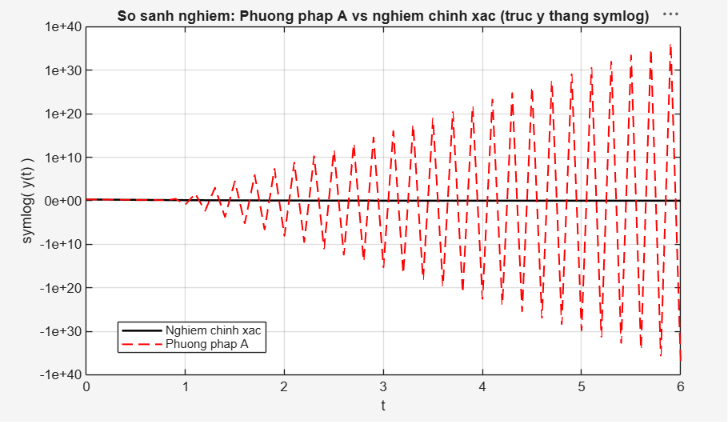
\includegraphics[width=\textwidth]{images/vd1_1.png}
    \caption{So sánh nghiệm số của phương pháp A và nghiệm chính xác. Trục tung sử dụng thang đo \texttt{symlog} (symmetric log).}
\end{figure}

\begin{figure}[H]
    \centering
    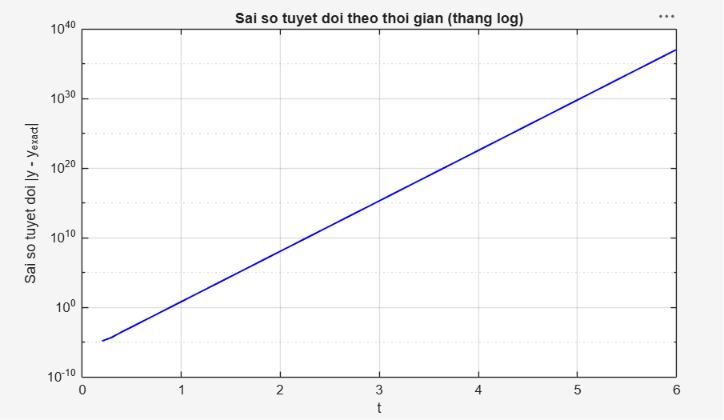
\includegraphics[width=\textwidth]{images/vd1_3.png}
    \caption{Đồ thị sai số của phương pháp A}
\end{figure}
\begin{table}[H]
\centering
\caption{So sánh nghiệm chính xác, nghiệm số của phương pháp A và sai số tuyệt đối tại một số thời điểm.}
\renewcommand{\arraystretch}{1.2}
\begin{tabular}{cccc}
\toprule
$t$ & $y_n$ & $Y_n$ & $E_n$\\
\midrule
0.0 & $1.000000\times10^{0}$  & $1.000000\times10^{0}$  & $0$\\
0.5 & $6.065307\times10^{-1}$ & $6.081996\times10^{-1}$ & $1.668921\times10^{-3}$\\
1.0 & $3.678794\times10^{-1}$ & $-6.677259\times10^{0}$ & $7.045138\times10^{0}$\\
2.0 & $1.353353\times10^{-1}$ & $-1.243391\times10^{8}$ & $1.243391\times10^{8}$\\
4.0 & $1.831564\times10^{-2}$ & $-3.872979\times10^{22}$ & $3.872979\times10^{22}$\\
6.0 & $2.478752\times10^{-3}$ & $-1.206376\times10^{37}$ & $1.206376\times10^{37}$\\
\bottomrule
\end{tabular}
\end{table}

\subsubsection*{Phân tích kết quả}

Kết quả thực nghiệm cho thấy trong những bước tính đầu tiên, nghiệm số của phương pháp A còn khá gần với nghiệm chính xác. Tuy nhiên, khi số bước lưới tăng lên, sai số bắt đầu tăng rất nhanh và nghiệm số nhanh chóng phân kỳ khỏi nghiệm đúng. Từ Bảng trên có thể thấy tại $t=1$, sai số đã đạt khoảng $7.05$, trong khi tại $t=6$ sai số lên tới khoảng $1.21\times10^{37}$.

Hiện tượng phân kỳ của phương pháp A có thể được giải thích trực tiếp thông qua nghiệm của phương trình sai phân tương ứng. Đối với bài toán
\[
y'(t)=-y(t),\qquad y(0)=1,
\]
ta có
\[
f_n=-Y_n.
\]

Thay vào công thức của phương pháp A thu được
\[
Y_{n+2}+4(1-h)Y_{n+1}-(5+2h)Y_n=0.
\]

Phương trình đặc trưng tương ứng là
\[
\lambda^2+4(1-h)\lambda-(5+2h)=0.
\]

Khi $h$ đủ nhỏ, hai nghiệm của phương trình đặc trưng có dạng
\[
\lambda_1=1+O(h),\qquad
\lambda_2=-5+O(h).
\]

Do đó nghiệm tổng quát của phương trình sai phân được biểu diễn dưới dạng
\[
Y_n=C_1\lambda_1^n+C_2\lambda_2^n,
\]
trong đó các hằng số $C_1,C_2$ phụ thuộc vào điều kiện ban đầu. Vì
\[
|\lambda_2|\approx5>1,
\]
thành phần $C_2\lambda_2^n$ được khuếch đại khoảng $5$ lần sau mỗi bước lặp. Mặc dù sai số ban đầu có thể rất nhỏ, thành phần này vẫn tăng theo cấp số nhân và nhanh chóng lấn át nghiệm thực của bài toán. Chính cơ chế khuếch đại này làm cho nghiệm số phân kỳ mặc dù phương pháp vẫn thỏa điều kiện nhất quán.

\subsection{Ví dụ 2}
\begin{vidu}{Ví dụ 2}
    Xét phương pháp đa bước tuyến tính hai bước, được gọi là \emph{phương pháp B}
    \begin{equation*}
        Y_{n+2}-4Y_{n+1}+3Y_n=-2h\,f_{n+2}.
    \end{equation*}
\end{vidu}


\subsubsection*{Kiểm tra tính nhất quán}

Một phương pháp đa bước tuyến tính được gọi là nhất quán nếu nó thỏa hai điều kiện sau: $\rho(1) = 0$ và $\rho'(1) = \sigma(1)$. Thay $z = 1$ vào $\rho(z)$:

$$ \rho(1) = 1^2 - 4(1) + 3 = 1 - 4 + 3 = 0 $$

$$ \rho'(z) = 2z - 4 \implies \rho'(1) = 2(1) - 4 = -2 $$

Tính giá trị của $\sigma(1)$:

$$ \sigma(1) = -2(1)^2 = -2 $$

Ta thấy $\rho(1) = 0$ và $\rho'(1) = \sigma(1) = -2$. Vậy phương pháp nhất quán.

\vspace{0.5cm}
\subsubsection*{Kiểm tra điều kiện nghiệm}

Đa thức đặc trưng thứ nhất:

\[
    \rho(z) = z^2 - 4z + 3 = (z - 1)(z - 3) = 0
\]  

\[
    z_1 = 1, \qquad z_2 = 3
\] 

Theo điều kiện nghiệm, mọi nghiệm của $\rho(z)$ phải có môđun không vượt quá 1, đồng thời các nghiệm nằm trên đường tròn đơn vị phải là nghiệm đơn. Tuy nhiên,
\[
|z_2| = 3 > 1, 
\]
nên phương pháp không thỏa điều kiện nghiệm. Theo Định lý Dahlquist, phương pháp không hội tụ.

\subsubsection*{Mô phỏng nghiệm số}

Nhằm minh họa cho các phân tích lý thuyết, phương pháp B được áp dụng để giải bài toán giá trị ban đầu:
\[
y'(t) = -y(t),\qquad y(0) = 1.
\]

Nghiệm chính xác của bài toán là $y(t) = e^{-t}$.

\begin{lstlisting}[style=MatlabStyle,caption={Mã MATLAB cho phương pháp B.},label={lst:methodB}]
clear; clc; close all;

% Thiet lap bai toan
f       = @(t, y) -y;          
y_exact = @(t) exp(-t);       
t0 = 0;
T  = 6;                       
h  = 0.1;                     
N  = round((T - t0) / h);
t  = t0 + (0:N) * h;

% Khoi tao
y = zeros(1, N + 1);
y(1) = y_exact(t(1));   % y0
y(2) = y_exact(t(2));   % y1

% Phuong phap B
for n = 1:(N - 1)
    y(n+2) = (4*y(n+1) - 3*y(n)) / (1 - 2*h);
end

% Nghiem chinh xac va sai so
yex = y_exact(t);
err = abs(y - yex);

% ---- In bang ket qua tai mot so moc thoi gian ----
moc = [0.0, 0.5, 1.0, 2.0, 4.0, 6.0];
fprintf('%8s %18s %18s %14s\n', 't', 'Nghiem chinh xac', 'Phuong phap', 'Sai so');
for k = 1:length(moc)
    [~, idx] = min(abs(t - moc(k)));
    fprintf('%8.1f %18.6e %18.6e %14.3e\n', t(idx), yex(idx), y(idx), err(idx));
end

thresh = 1;
symlog = @(x) sign(x) .* log10(1 + abs(x) / thresh);

% ---- Do thi ----

% Hinh 1: Thang symlog
figure(1);
plot(t, symlog(yex), 'k-', 'LineWidth', 1.5); hold on;
plot(t, symlog(y),   'r--', 'LineWidth', 1.2);
legend('Nghiem chinh xac', 'Phuong phap B', 'Location', 'best');
xlabel('t'); ylabel('symlog( y(t) )');
title('Hinh 1: Phuong phap B vs Nghiem chinh xac (truc y thang symlog)');
grid on;

% Ve lai nhan truc tung theo gia tri that (chi de doc so, khong anh huong tinh toan)
yt = get(gca, 'YTick');
yticklabels_real = arrayfun(@(v) sprintf('%.0e', sign(v)*(10^abs(v)-1)*thresh), yt, 'UniformOutput', false);
set(gca, 'YTickLabel', yticklabels_real);

% Hinh 2: Thang binh thuong
figure(2);
plot(t, yex, 'k-', 'LineWidth', 1.5); hold on;
plot(t, y,   'r--', 'LineWidth', 1.2);
legend('Nghiem chinh xac', 'Phuong phap B', 'Location', 'best');
xlabel('t'); ylabel('y(t)');
title('Hinh 2: Phuong phap B va Nghiem chinh xac');
grid on;

% Hinh 3: Thang log cho sai so
figure(3);
semilogy(t, err, 'b-', 'LineWidth', 1.2);
xlabel('t'); ylabel('Sai so tuyet doi |y - y_{exact}|');
title('Hinh 3: Sai so tuyet doi theo thoi gian (thang log)');
grid on;
\end{lstlisting}
\begin{figure}[H]
    \centering
    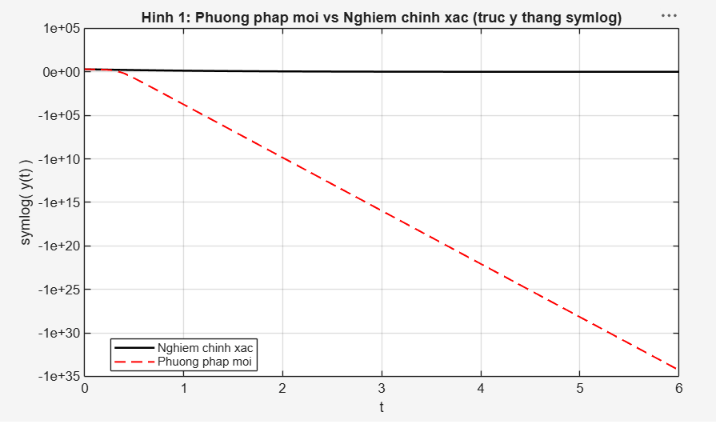
\includegraphics[width=\textwidth]{images/vd2_1.png}
    \caption{So sánh nghiệm số của phương pháp B và nghiệm chính xác. Trục tung sử dụng thang đo \texttt{symlog} (symmetric log).}
\end{figure}

\begin{figure}[H]
    \centering
    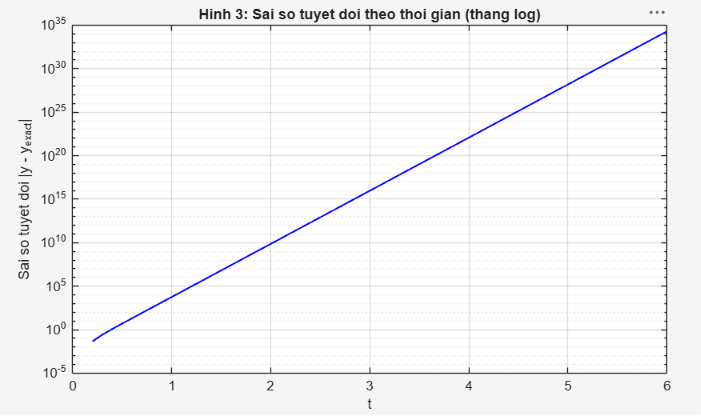
\includegraphics[width=\textwidth]{images/vd2_3.png}
    \caption{Đồ thị sai số của phương pháp B}
\end{figure}
\begin{table}[H]
\centering
\caption{So sánh nghiệm chính xác, nghiệm số của phương pháp B và sai số tuyệt đối tại một số thời điểm.}
\renewcommand{\arraystretch}{1.2}
\begin{tabular}{cccc}
\toprule
$t$ & $y_n$ & $Y_n$ & $E_n$\\
\midrule
0.0 & 1.000000e+00 & \phantom{-}1.000000e+00 & 0 \\
0.5 & 6.065307e-01 & -4.362861e+00 & 4.969e+00 \\
1.0 & 3.678794e-01 & -5.683881e+03 & 5.684e+03 \\
2.0 & 1.353353e-01 & -7.286041e+09 & 7.286e+09 \\
4.0 & 1.831564e-02 & -1.197068e+22 & 1.197e+22 \\
6.0 & 2.478752e-03 & -1.966737e+34 & 1.967e+34 \\
\bottomrule
\end{tabular}
\end{table}

\subsubsection*{Phân tích kết quả}

Kết quả mô phỏng cho thấy phương pháp B cũng không cho nghiệm hội tụ về nghiệm chính xác. Ngay từ những bước tính đầu tiên, sai số đã tăng nhanh và tiếp tục khuếch đại theo thời gian. Từ Bảng trên có thể thấy sai số tại $t=0.5$ đã đạt gần $5$, và đến $t=6$ đạt xấp xỉ $1.97\times10^{34}$.

Hiện tượng phân kỳ của phương pháp B cũng có thể được giải thích thông qua nghiệm của phương trình sai phân tương ứng. Đối với bài toán
\[
y'(t)=-y(t),\qquad y(0)=1,
\]
ta có
\[
f_{n+2}=-Y_{n+2}.
\]

Thay vào công thức của phương pháp B thu được
\[
(1-2h)Y_{n+2}-4Y_{n+1}+3Y_n=0.
\]

Phương trình đặc trưng tương ứng là
\[
(1-2h)\lambda^2-4\lambda+3=0.
\]

Khi $h$ đủ nhỏ, hai nghiệm của phương trình đặc trưng có dạng
\[
\lambda_1=1+O(h),\qquad
\lambda_2=3+O(h).
\]

Do đó nghiệm tổng quát của phương trình sai phân được biểu diễn dưới dạng
\[
Y_n=C_1\lambda_1^n+C_2\lambda_2^n,
\]
trong đó các hằng số $C_1,C_2$ phụ thuộc vào điều kiện ban đầu. Vì
\[
|\lambda_2|\approx3>1,
\]
thành phần $C_2\lambda_2^n$ được khuếch đại xấp xỉ $3$ lần sau mỗi bước lặp. Mặc dù sai số ban đầu có thể rất nhỏ, thành phần này vẫn tăng theo cấp số nhân và nhanh chóng lấn át nghiệm thực của bài toán. Chính cơ chế khuếch đại này làm cho nghiệm số phân kỳ mặc dù phương pháp vẫn thỏa điều kiện nhất quán.

\subsubsection*{Tóm tắt}
Hai ví dụ thực nghiệm trong chương này đã minh họa trực quan các kết quả của định lý Dashquist. Ví dụ 1 khảo sát một phương pháp đa bước tuyến tính hiện, trong khi Ví dụ 2 khảo sát một phương pháp đa bước tuyến tính ẩn. Mặc dù cả hai phương pháp đều thỏa điều kiện nhất quán, chúng đều vi phạm điều kiện nghiệm. Kết quả là sai số không bị triệt tiêu mà ngược lại còn được khuếch đại sau mỗi bước lặp, khiến nghiệm số nhanh chóng phân kỳ khỏi nghiệm chính xác.

Các bảng số liệu và đồ thị MATLAB đều cho thấy sai số tăng rất nhanh theo thời gian, hoàn toàn phù hợp với phân tích lý thuyết dựa trên điều kiện 0-ổn định. Điều này xác nhận rằng tính nhất quán chỉ là điều kiện cần, còn tính 0-ổn định mới là điều kiện quyết định để đảm bảo hội tụ của phương pháp đa bước tuyến tính.

Qua các ví dụ trên có thể rút ra rằng việc lựa chọn một phương pháp số không chỉ dựa trên bậc chính xác hay việc phương pháp là hiện hoặc ẩn, mà quan trọng hơn là phải kiểm tra điều kiện nghiệm của đa thức đặc trưng. Đây cũng chính là nội dung cốt lõi của Định lý hội tụ Dahlquist và cũng là cơ sở lý thuyết cho việc xây dựng các phương pháp ổn định trong thực tế.